\PassOptionsToPackage{unicode=true}{hyperref} % options for packages loaded elsewhere
\PassOptionsToPackage{hyphens}{url}
%
\documentclass[english,man,floatsintext]{apa6}
\usepackage{lmodern}
\usepackage{amssymb,amsmath}
\usepackage{ifxetex,ifluatex}
\usepackage{fixltx2e} % provides \textsubscript
\ifnum 0\ifxetex 1\fi\ifluatex 1\fi=0 % if pdftex
  \usepackage[T1]{fontenc}
  \usepackage[utf8]{inputenc}
  \usepackage{textcomp} % provides euro and other symbols
\else % if luatex or xelatex
  \usepackage{unicode-math}
  \defaultfontfeatures{Ligatures=TeX,Scale=MatchLowercase}
\fi
% use upquote if available, for straight quotes in verbatim environments
\IfFileExists{upquote.sty}{\usepackage{upquote}}{}
% use microtype if available
\IfFileExists{microtype.sty}{%
\usepackage[]{microtype}
\UseMicrotypeSet[protrusion]{basicmath} % disable protrusion for tt fonts
}{}
\IfFileExists{parskip.sty}{%
\usepackage{parskip}
}{% else
\setlength{\parindent}{0pt}
\setlength{\parskip}{6pt plus 2pt minus 1pt}
}
\usepackage{hyperref}
\hypersetup{
            pdftitle={multibridge: An R Package To Evaluate Multinomial Order Constraints},
            pdfauthor={Alexandra Sarafoglou1, Julia M. Haaf1, Frederik Aust1, Eric-Jan Wagenmakers1, \& Maarten Marsman1},
            pdfborder={0 0 0},
            breaklinks=true}
\urlstyle{same}  % don't use monospace font for urls
\usepackage{color}
\usepackage{fancyvrb}
\newcommand{\VerbBar}{|}
\newcommand{\VERB}{\Verb[commandchars=\\\{\}]}
\DefineVerbatimEnvironment{Highlighting}{Verbatim}{commandchars=\\\{\}}
% Add ',fontsize=\small' for more characters per line
\usepackage{framed}
\definecolor{shadecolor}{RGB}{248,248,248}
\newenvironment{Shaded}{\begin{snugshade}}{\end{snugshade}}
\newcommand{\AlertTok}[1]{\textcolor[rgb]{0.94,0.16,0.16}{#1}}
\newcommand{\AnnotationTok}[1]{\textcolor[rgb]{0.56,0.35,0.01}{\textbf{\textit{#1}}}}
\newcommand{\AttributeTok}[1]{\textcolor[rgb]{0.77,0.63,0.00}{#1}}
\newcommand{\BaseNTok}[1]{\textcolor[rgb]{0.00,0.00,0.81}{#1}}
\newcommand{\BuiltInTok}[1]{#1}
\newcommand{\CharTok}[1]{\textcolor[rgb]{0.31,0.60,0.02}{#1}}
\newcommand{\CommentTok}[1]{\textcolor[rgb]{0.56,0.35,0.01}{\textit{#1}}}
\newcommand{\CommentVarTok}[1]{\textcolor[rgb]{0.56,0.35,0.01}{\textbf{\textit{#1}}}}
\newcommand{\ConstantTok}[1]{\textcolor[rgb]{0.00,0.00,0.00}{#1}}
\newcommand{\ControlFlowTok}[1]{\textcolor[rgb]{0.13,0.29,0.53}{\textbf{#1}}}
\newcommand{\DataTypeTok}[1]{\textcolor[rgb]{0.13,0.29,0.53}{#1}}
\newcommand{\DecValTok}[1]{\textcolor[rgb]{0.00,0.00,0.81}{#1}}
\newcommand{\DocumentationTok}[1]{\textcolor[rgb]{0.56,0.35,0.01}{\textbf{\textit{#1}}}}
\newcommand{\ErrorTok}[1]{\textcolor[rgb]{0.64,0.00,0.00}{\textbf{#1}}}
\newcommand{\ExtensionTok}[1]{#1}
\newcommand{\FloatTok}[1]{\textcolor[rgb]{0.00,0.00,0.81}{#1}}
\newcommand{\FunctionTok}[1]{\textcolor[rgb]{0.00,0.00,0.00}{#1}}
\newcommand{\ImportTok}[1]{#1}
\newcommand{\InformationTok}[1]{\textcolor[rgb]{0.56,0.35,0.01}{\textbf{\textit{#1}}}}
\newcommand{\KeywordTok}[1]{\textcolor[rgb]{0.13,0.29,0.53}{\textbf{#1}}}
\newcommand{\NormalTok}[1]{#1}
\newcommand{\OperatorTok}[1]{\textcolor[rgb]{0.81,0.36,0.00}{\textbf{#1}}}
\newcommand{\OtherTok}[1]{\textcolor[rgb]{0.56,0.35,0.01}{#1}}
\newcommand{\PreprocessorTok}[1]{\textcolor[rgb]{0.56,0.35,0.01}{\textit{#1}}}
\newcommand{\RegionMarkerTok}[1]{#1}
\newcommand{\SpecialCharTok}[1]{\textcolor[rgb]{0.00,0.00,0.00}{#1}}
\newcommand{\SpecialStringTok}[1]{\textcolor[rgb]{0.31,0.60,0.02}{#1}}
\newcommand{\StringTok}[1]{\textcolor[rgb]{0.31,0.60,0.02}{#1}}
\newcommand{\VariableTok}[1]{\textcolor[rgb]{0.00,0.00,0.00}{#1}}
\newcommand{\VerbatimStringTok}[1]{\textcolor[rgb]{0.31,0.60,0.02}{#1}}
\newcommand{\WarningTok}[1]{\textcolor[rgb]{0.56,0.35,0.01}{\textbf{\textit{#1}}}}
\usepackage{graphicx,grffile}
\makeatletter
\def\maxwidth{\ifdim\Gin@nat@width>\linewidth\linewidth\else\Gin@nat@width\fi}
\def\maxheight{\ifdim\Gin@nat@height>\textheight\textheight\else\Gin@nat@height\fi}
\makeatother
% Scale images if necessary, so that they will not overflow the page
% margins by default, and it is still possible to overwrite the defaults
% using explicit options in \includegraphics[width, height, ...]{}
\setkeys{Gin}{width=\maxwidth,height=\maxheight,keepaspectratio}
\setlength{\emergencystretch}{3em}  % prevent overfull lines
\providecommand{\tightlist}{%
  \setlength{\itemsep}{0pt}\setlength{\parskip}{0pt}}
\setcounter{secnumdepth}{0}

% set default figure placement to htbp
\makeatletter
\def\fps@figure{htbp}
\makeatother

% Manuscript styling
\usepackage{upgreek}
\captionsetup{font=singlespacing,justification=justified}

% Table formatting
\usepackage{longtable}
\usepackage{lscape}
% \usepackage[counterclockwise]{rotating}   % Landscape page setup for large tables
\usepackage{multirow}		% Table styling
\usepackage{tabularx}		% Control Column width
\usepackage[flushleft]{threeparttable}	% Allows for three part tables with a specified notes section
\usepackage{threeparttablex}            % Lets threeparttable work with longtable

% Create new environments so endfloat can handle them
% \newenvironment{ltable}
%   {\begin{landscape}\begin{center}\begin{threeparttable}}
%   {\end{threeparttable}\end{center}\end{landscape}}
\newenvironment{lltable}{\begin{landscape}\begin{center}\begin{ThreePartTable}}{\end{ThreePartTable}\end{center}\end{landscape}}

% Enables adjusting longtable caption width to table width
% Solution found at http://golatex.de/longtable-mit-caption-so-breit-wie-die-tabelle-t15767.html
\makeatletter
\newcommand\LastLTentrywidth{1em}
\newlength\longtablewidth
\setlength{\longtablewidth}{1in}
\newcommand{\getlongtablewidth}{\begingroup \ifcsname LT@\roman{LT@tables}\endcsname \global\longtablewidth=0pt \renewcommand{\LT@entry}[2]{\global\advance\longtablewidth by ##2\relax\gdef\LastLTentrywidth{##2}}\@nameuse{LT@\roman{LT@tables}} \fi \endgroup}

% \setlength{\parindent}{0.5in}
% \setlength{\parskip}{0pt plus 0pt minus 0pt}

% \usepackage{etoolbox}
\makeatletter
\patchcmd{\HyOrg@maketitle}
  {\section{\normalfont\normalsize\abstractname}}
  {\section*{\normalfont\normalsize\abstractname}}
  {}{\typeout{Failed to patch abstract.}}
\patchcmd{\HyOrg@maketitle}
  {\section{\protect\normalfont{\@title}}}
  {\section*{\protect\normalfont{\@title}}}
  {}{\typeout{Failed to patch title.}}
\makeatother
\shorttitle{multibridge}
\DeclareDelayedFloatFlavor{ThreePartTable}{table}
\DeclareDelayedFloatFlavor{lltable}{table}
\DeclareDelayedFloatFlavor*{longtable}{table}
\makeatletter
\renewcommand{\efloat@iwrite}[1]{\immediate\expandafter\protected@write\csname efloat@post#1\endcsname{}}
\makeatother
\usepackage{lineno}

\linenumbers
\usepackage{csquotes}
\usepackage{bm}
\usepackage{amsmath}
\usepackage{nicefrac}
\usepackage{caption}
\usepackage{xcolor}
\definecolor{mypink}{RGB}{255, 230, 255}
\definecolor{myWheat}{RGB}{245, 222, 179}
\usepackage{todonotes}
\newcommand{\Julia}[1]{\todo[inline, color=mypink]{#1}}
\newcommand{\Frederik}[1]{\todo[inline, color=myWheat]{#1}}
\ifnum 0\ifxetex 1\fi\ifluatex 1\fi=0 % if pdftex
  \usepackage[shorthands=off,main=english]{babel}
\else
  % load polyglossia as late as possible as it *could* call bidi if RTL lang (e.g. Hebrew or Arabic)
  \usepackage{polyglossia}
  \setmainlanguage[]{english}
\fi

\title{multibridge: An R Package To Evaluate Multinomial Order Constraints}
\author{Alexandra Sarafoglou\textsuperscript{1}, Julia M. Haaf\textsuperscript{1}, Frederik Aust\textsuperscript{1}, Eric-Jan Wagenmakers\textsuperscript{1}, \& Maarten Marsman\textsuperscript{1}}
\date{}


\affiliation{\vspace{0.5cm}\textsuperscript{1} University of Amsterdam}

\abstract{
The \textbf{multibridge} package has been developed to efficiently compute Bayes factors for binomial and multinomial models, that feature inequality constraints, equality constrains and free parameters. By using the bridge sampling algorithm to compute the Bayes factor, \textbf{multibridge} facilitates the evaluation of large models with many constraints and models with very small parameter spaces. The package was developed in the R programming language and is freely available from the Comprehensive \texttt{R} Archive Network. We illustrate the functions based on two empirical examples.
}



\begin{document}
\maketitle

\hypertarget{introduction}{%
\section{Introduction}\label{introduction}}

\todo[inline, color=mypink]{I would first mention for which models the package is, multinomial and binomial and then then constraints.}

We present \textbf{multibridge}, an \texttt{R} package to evaluate informed hypotheses on category variables using Bayesian inference. This package allows users to specify constraints on the underlying category proportions including inequality constraints, equality constraints, free parameters and mixtures between them. This package is available from the Comprehensive \texttt{R} Archive Network (CRAN) at \url{https://CRAN.R-project.org/package=multibridge}. Here we introduce the methodology used to evaluate informed hypotheses in multinomial models and models featuring independent binomials and show how to use the implementations provided in \textbf{multibridge} through fully reproducible examples.

The most common way to analyze categorial variables is to test whether the underlying category proportions are exactly equal or whether they are fixed and follow a predicted pattern. Often however, scientific hypotheses go beyond this standard case and predict for instance ordinal relations among the underlying category proportions, such as increasing or decreasing trends. For instance, to check for irregularities in audit data, one could test whether the leading digits in the data are distributed according to an expected Benford distribution or whether they deviate from it by, for example, showing a general decreasing trend. Informed hypotheses could also feature combinations of equality and inequality constrained parameters, as well as parameters that are free to vary. For instance, when studying the prevalence of statistical reporting errors in articles published in different areas of psychological science, one could hypothesize that articles published in social psychology journals have higher error rates than articles published in other psychological journals while not expressing expectations about the error rate distribution among these other journals (Nuijten, Hartgerink, Assen, Epskamp, \& Wicherts, 2016). Generally, testing informed hypotheses allows researchers to specify hypotheses that follow more closely relate to their theories.

\todo[inline, color=mypink]{I really like the paragraph below. But I think we have to motivate it a bit better. How do you get from the paragraph above to this one?}

For the \textbf{multibridge} package the emphasis is on the approximation of Bayes factors (Jeffreys, 1935; Kass \& Raftery, 1995) to quantify evidence for or against informative models. In the \texttt{R} programming language, the package \textbf{multinomineq} (Heck \& Davis-Stober, 2019) is available to evaluate order constrained hypotheses for multinomial models as well as models that feature independent binomials. \textbf{multinomineq} allows users to specify inequality constrained hypotheses but also more general linear inequality constraints. The \texttt{BAIN} (Gu, Hoijtink, Mulder, \& Rosseel, 2019) package allows for the evaluation of inequality constraints in structural equation models. Outside of \texttt{R}, the software package \texttt{BIEMS} (Mulder, Hoijtink, Leeuw, \& others, 2012) allows for the evaluation of order constraints for multivariate linear models such as MANOVA, repeated measures, and multivariate regression. \todo[inline, color=mypink]{Which language is it? Or is it a GUI?} All these packages rely on two popular methods to approximate order constrained Bayes factors, the encompassing prior approach (Gu, Mulder, Deković, \& Hoijtink, 2014; Hoijtink, 2011; Hoijtink, Klugkist, \& Boelen, 2008; Klugkist, Kato, \& Hoijtink, 2005) and the conditioning method (Mulder, 2014, 2016; Mulder et al., 2009). But even though these methods are currently very popular and widely used, they are shown to become increasingly unreliable and inefficient as the number of constraints increases or when the parameter space of the constrained model is small (Sarafoglou et al., 2020).

The \textbf{multibridge} uses a bridge sampling routine that enables users to compute Bayes factors for informed hypotheses more reliably and efficiently (Bennett, 1976; Meng \& Wong, 1996; Sarafoglou et al., 2020). The workhorse for this analysis, the bridge sampling algorithm, constitutes a special case of the algorithm implemented in the \texttt{R} package \textbf{bridgesampling} (Gronau, Singmann, \& Wagenmakers, 2020). With \textbf{bridgesampling}, users are able to estimate the marginal likelihood for a wide variety of models, including models implemented in Stan (Stan Development Team, 2020). However, \textbf{bridgesampling} is not suitable for models that include constraints on probability vectors. In \textbf{multibridge}, we tailored the bridge sampling algorithm such that it accommodates the specification of informed hypotheses on probability vectors. The general workflow of \textbf{multibridge} is illustrated in Figure \ref{fig:scheme-multibridge}.



\begin{figure}
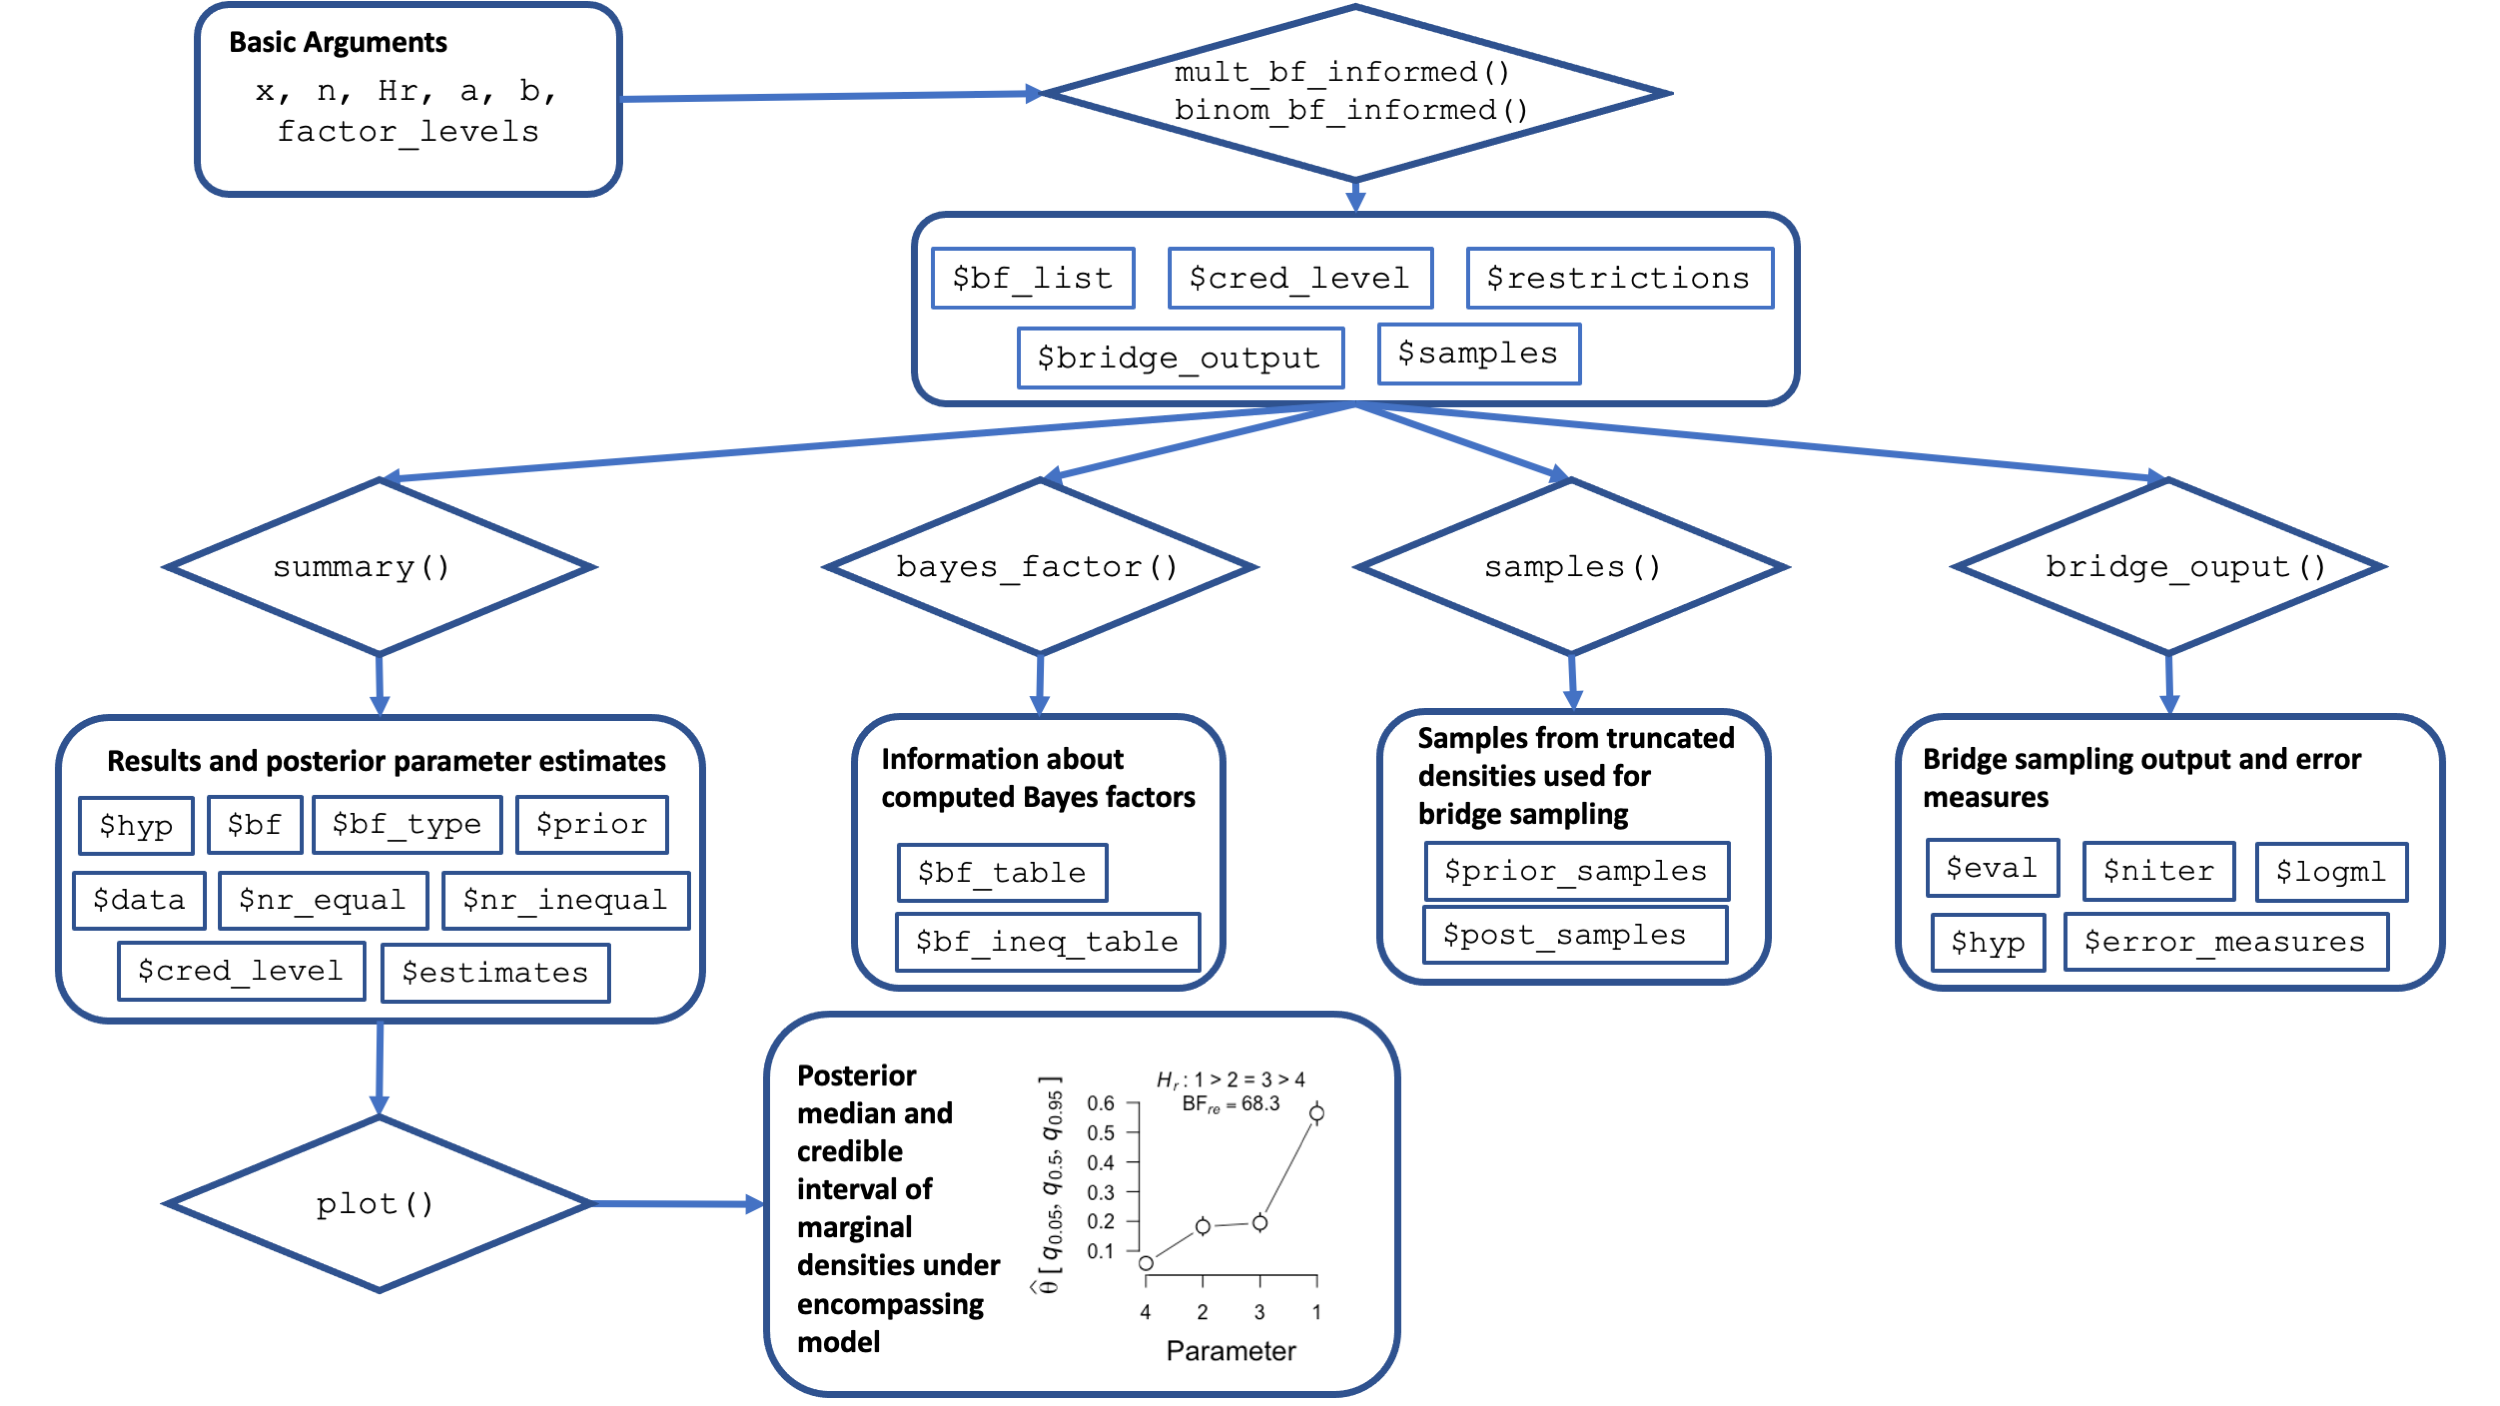
\includegraphics[width=400px]{scheme_multibridge} \caption[(fig:scheme-multibridge)]{The \textbf{multibridge} workflow. The user needs to specify the data values (\texttt{x} and \texttt{n} for binomial models and \texttt{x} for multinomial models, respectively), the informed hypothesis (\texttt{Hr}), the \(\alpha\) and \(\beta\) parameters of the Binomial prior distributions (\texttt{a} and \texttt{b}) or the concentration parameters for the Dirichlet prior distribution (\texttt{a}), respectively, and the factor levels (\texttt{factor\_levels}). The functions \texttt{multBfInformed} and \texttt{binomBfInformed} then produce an estimate for the Bayes factor of the informed hypothesis versus the encompassing hypothesis in which all parameters are free to vary. Based on these results different S3 methods can be used to get more detailed information on the individual components of the analysis (\texttt{summary}, (\textbackslash{}texttt\{bayes\_factor\}), and parameter estimates of the encompassing distribution (\texttt{plot}).}\label{fig:scheme-multibridge}
\end{figure}

The two core functions of \textbf{multibridge} --the \texttt{multBfInformed}-function and the \texttt{binomBfInformed}-function -- can be illustrated schematically as follows:

\begin{Shaded}
\begin{Highlighting}[]
\KeywordTok{multBfInformed}\NormalTok{(x, Hr, a factor_levels)}
\KeywordTok{binomBfInformed}\NormalTok{(x, n, Hr, a, b, factor_levels)}
\end{Highlighting}
\end{Shaded}

The basic required arguments for these functions are listed in Table \ref{tab:arguments}.

\begin{table}
\caption{To estimate the Bayes factor in favor for or against the specified informed hypothesis, the user provides the core functions \texttt{multBfInformed} and \texttt{binomBfInformed} with the following basic required arguments}
\label{tab:arguments}
\begin{center}
\begin{tabular}{p{4cm}p{12cm}}
        \toprule
Argument & Description \\\midrule
\texttt{x} & a vector with data (for multinomial models) or a vector of counts of successes, or a two-dimensional table (or matrix) with 2 columns, giving the counts of successes and failures, respectively (for binomial models)  \\
\texttt{n} &  numeric. Vector of counts of trials. Must be the same length as \texttt{x}. Ignored if \texttt{x} is a matrix or a table \\
\texttt{Hr} & string or character. Encodes the user specified informed hypothesis. Users can either use the specified \texttt{factor\_levels} or indexes to refer to parameters.\\
\texttt{a} & numeric. Vector with concentration parameters of Dirichlet distribution (for multinomial models) or alpha parameters for independent beta distributions (for binomial models). Default sets all parameters to 1 \\
\texttt{b} & numeric. Vector with beta parameters. Must be the same length as \texttt{x}. Default sets all beta parameters to 1 \\
\texttt{factor\_levels} &  character. Vector with category names. Must be the same length as \texttt{x}\\
\bottomrule
\end{tabular}
\end{center}
\end{table}

The package produces an estimate for the Bayes factor in favor of or against the informed hypothesis. The resulting Bayes factor compares the evidence for the informed hypotheses to the encompassing hypothesis that imposes no constraints on the underlying category proportions. Given this result, the user can then either receive a visualization of the prior and posterior parameter estimates using the \texttt{plot}-method, or get more detailed information on how the Bayes factors is composed using the \texttt{summary}-method. For hypotheses that include mixtures between equality and inequality informed hypotheses the \texttt{bayes\_factor} method shows the conditional Bayes factor for the inequality constraints given the equality constraints and a Bayes factor for the equality constraints. Table \ref{table:s3_methods} summarizes all S3 methods currently implemented in \textbf{multibridge}.

\begin{table}
\caption {S3 methods implemented in $\textbf{multibridge}$}
\label{table:s3_methods}
\begin{center}
\begin{tabular}{p{4cm}p{3.5cm}p{9cm}}
        \toprule
Function Name(s) & S3 Method & Description \\\midrule
$\texttt{multBfInformed}$, $\texttt{binomBfInformed}$ & $\texttt{print}$ & Prints model specifications and descriptives. \\
 & $\texttt{summary}$ &  Prints and returns the Bayes factor and associated hypotheses for the full model, and all equality and inequality constraints.\\
  & $\texttt{plot}$ &  Plots the posterior median and credible interval of the parameter estimates of the encompassing model.\\
 & $\texttt{bayes\_factor}$ & Contains all Bayes factors and log marginal likelihood estimates for inequality constraints.\\
 & $\texttt{samples}$ & Extracts prior and posterior samples from constrained distribution (if bridge sampling was applied). \\
& $\texttt{bridge\_output}$    &  Extracts bridge sampling output and associated error measures.\\
& $\texttt{restriction\_list}$ & Extracts restriction list and associated informed hypothesis. \\
$\texttt{binomBfInequality}$, $\texttt{binomBfInequality}$  & $\texttt{print}$ & Prints the bridge sampling estimate for the log marginal likelihood and the corresponding percentage error. \\
& $\texttt{summary}$ & Prints and returns the bridge sampling estimate for the log marginal likelihood and associated error terms.\\
\bottomrule
\end{tabular}
\end{center}
\end{table}

This remainder of this article is organized as follows: In the methods section, we describe the Bayes factor identity for informed hypotheses in binomial and multinomial models, and present the bridge sampling routine implemented in the \textbf{multibridge} package including details of the necessary transformations required for this routine. In Section 3, we will schematically introduce the most relevant functions in \textbf{multibridge} and their arguments. Section 4 illustrates how to use the \textbf{multibridge} package to estimate parameters, and compute Bayes factors using two examples.

\todo[inline, color=mypink]{stopped here.}

\hypertarget{methods}{%
\section{Methods}\label{methods}}

\textbf{multibridge} allows users to specify informed hypotheses in multinomial models and models that feature independent binomial probabilities. In the multinomial model, twe assumes that the vector of observations \(x_1, \cdots, x_K\) in the \(K\) categories follow a multinomial distribution. The parameter vector of the multinomial model, \(\theta_1, \cdots, \theta_K\), contains the probabilities of observing a value in a particular category. The parameter vector \(\theta_1, \cdots, \theta_K\) is drawn from a Dirichlet distribution with concentration parameters \(\alpha_1, \cdots, \alpha_K\). Formally, the model can be described as follows:

\begin{align}
  x_1, \cdots, x_K &\sim \text{Multinomial}(\sum_{k = 1}^K x_k, \theta_1, \cdots, \theta_K) \\
  \theta_1, \cdots, \theta_K &\sim \text{Dirichlet}(\alpha_1, \cdots, \alpha_K). \\
\end{align}

In the binomial model we assume that the elements in the vector of successes \(x_1, \cdots, x_K\) and the elements in the vector of total number of observations \(n_1, \cdots, n_K\) in the \(K\) categories follow independent binomial distributions. As in the multinomial model, the parameter vector of the binomial success probabilities, \(\theta_1, \cdots, \theta_K\), contains the probabilities of observing a value in a particular category. The parameter vector \(\theta_1, \cdots, \theta_K\) are drawn from independent beta distributions with parameters \(\alpha_1, \cdots, \alpha_K\) and \(\beta_1, \cdots, \beta_K\). The model can be described as follows:

\begin{align}
  x_1 \cdots x_K & \sim \prod_{k = 1}^K \text{Binomial}(\theta_k, n_k) \\
  \theta_1 \cdots \theta_K &\sim \prod_{k = 1}^K \text{Beta}(\alpha_k, beta_k) \\
\end{align}

\hypertarget{bayes-factor}{%
\subsection{Bayes factor}\label{bayes-factor}}

When evaluating informed hypotheses that feature mixtures between inequality and equality constraints it is important to realize that the Bayes factor, further denoted as \(\text{BF}_{me}\), factors follows:

\[
\text{BF}_{me}
= \text{BF}_{0e} \times \text{BF}_{re} \mid \text{BF}_{0e},
\]
where the subscript \(m\) denotes a hypothesis that features mixtures of inequality and equality constraints. A Bayes factor for mixtures thus factors into a Bayes factor for the equality constraints, \(\text{BF}_{0e}\), and a conditional Bayes factor for the inequality constraints given the equality constraints \(\text{BF}_{re} \mid \text{BF}_{0e}\).

\hypertarget{the-bayes-factor-for-equality-constraints}{%
\subsection{The Bayes Factor For Equality Constraints}\label{the-bayes-factor-for-equality-constraints}}

For binomial models, the (marginal) Bayes factor for the equality constraints can be computed analytically and implemented in the function \texttt{binomBfEquality}. Assuming that the first \(i\) binomial probabilities in a model are equality constraint, the Bayes factor\(\text{BF}_{0e}\) is defined as:
\begin{align*}
\text{BF}_{0e} &=
&= \cfrac{\prod_{i < k} \text{B}(\alpha_i\text{, } \beta_i)}{\prod_{i < k} \text{B}(\alpha_i + x_i\text{, } \beta_i + n_i - x_i)} \times \cfrac{\text{B}(\alpha_+ + x_+ - i + 1\text{, } \beta_+ + n_+ - x_+ - i + 1)}{\text{B}(\alpha_+ - i + 1\text{, } - i + 1)}
\end{align*}
where \(\sum_{i<k}\alpha_i = \alpha_+\), \(\sum_{i<k}\beta_i = \beta_+\), \(\sum_{i<k} x_i = x_+\) and \(\sum_{i<k} n_i = n_+\). The latter factor introduces a correction for marginalizing which stems from the change in degrees of freedom, when we collapse \(i\) equality constraint parameters, that is, for \(i\) collapsed categories, \(i - 1\) degrees of freedom are lost which are subtracted from the prior parameters in the corresponding Binomial distribution.

For multinomial models, the (marginal) Bayes factor for the equality constraints is also analytically available and implemented in the function \texttt{multBayesBfEquality}. Assuming again that the first \(i\) category probabilities in a model are equality constraint, the Bayes factor\(\text{BF}_{0e}\) is defined as:
\begin{align*}
\text{BF}_{e0} = \frac{\text{B}(\boldsymbol{\alpha})}{\text{B}(\boldsymbol{\alpha}+\mathbf{x})} \, \left(\frac{1}{i}\right)^{\sum_{i<k} x_i}\,\frac{\text{B}\left(\sum_{i<k}\alpha_i+x_i - i + 1\text{, }\alpha_{k}+x_{k}\text{, }\dots\text{, }\alpha_K+x_K\right)}{
 \text{B}\left(\sum_{i<k}\alpha_i - i + 1\text{, }\alpha_{k}\text{, }\dots\text{, }\alpha_K\right)},
\end{align*}

\hypertarget{the-bayes-factor-for-inequality-constraints}{%
\subsection{The Bayes Factor For Inequality Constraints}\label{the-bayes-factor-for-inequality-constraints}}

For inequality constrained hypotheses, Klugkist et al. (2005) has derived the following identity of
the Bayes factor \(\text{BF}_{re}\):

\begin{align}
\label{Eq:klugkistIdentity}
\text{BF}_{re} &= \cfrac{\overbrace{p(\boldsymbol{\theta} \in \mathcal{R}_r \mid \mathbf{x}\text{, }\mathcal{H}_e)}^{\substack{\text{Proportion of posterior parameter}\\\text{space consistent with the restriction}}}}{\underbrace{p(\boldsymbol{\theta} \in \mathcal{R}_r \mid  \mathcal{H}_e)}_{\substack{\text{Proportion of prior parameter}\\\text{space consistent with the restriction}}}},
\end{align}

where in \(\text{BF}_{re}\), the subscript \(r\) denotes the inequality constrained hypothesis and the subscript \(e\) denotes the encompassing hypothesis that lets all parameters free to vary. Recently, however, Sarafoglou et al. (2020) showed that the Bayes factor \(\text{BF}_{re}\) can also be interpreted as ratio of two marginal likelihoods:

\begin{align}
\label{Eq:sarafoglouIdentity}
\text{BF}_{re} =
\cfrac{\overbrace{p(\boldsymbol{\theta} \in \mathcal{R}_r \mid \mathbf{x}\text{, }\mathcal{H}_e)}^{\substack{\text{Marginal likelihood of}\\\text{posterior distribution}}}}{\underbrace{p(\boldsymbol{\theta} \in \mathcal{R}_r \mid  \mathcal{H}_e)}_{\substack{\text{Marginal likelihood of}\\\text{prior distribution}}}}.
\end{align}

In this identity, \(p(\boldsymbol{\theta} \in \mathcal{R}_r \mid \mathbf{x}\text{, }\mathcal{H}_e)\) denotes the marginal likelihood of the constrained posterior distribution and \(p(\boldsymbol{\theta} \in \mathcal{R}_r \mid \mathcal{H}_e)\) denotes the marginal likelihood of the constrained prior distribution. Even though both identities are mathematically equivalent, the methods to estimate these identities are very different.
In the first case, for instance, the number of samples from the encompassing distribution in accordance with the inequality constrained hypothesis, serve as an estimate for the proportion of prior parameter space consistent with the restriction. On the flip side, however, this means that the accuracy of this estimate is strongly dependent on the number of the constrained parameters in the model and the size of the constrained parameter space. That is, the smaller the constrained parameter space is, the less likely it is that draws from the encompassing distribution will fall in this region, so that in some cases the estimation of the Bayes factor becomes practically impossible (Sarafoglou et al., 2020).

However, when we interpret the Bayes factor \(\text{BF}_{re}\) as ratio of marginal likelihoods and we are able to sample from the constrained prior and posterior distributions, numerical sampling methods such as bridge sampling to obtain the estimates. Crucially, in this approach, it does not matter how small the constrained parameter space is in proportion to the encompassing density. This gives the method a decisive advantage in terms of accuracy and efficiency.

\hypertarget{the-bridge-sampling-method}{%
\subsection{The Bridge Sampling Method}\label{the-bridge-sampling-method}}

Bridge sampling is a method to estimate the ratio of two marginal likelihoods which yield the Bayes factor (Bennett, 1976; Meng \& Wong, 1996). In the \textbf{multibridge} package we implemented a version of bridge sampling that estimates one marginal likelihood at the time since it increases the accuracy of the method without considerably increasing its computational efficiency (Overstall \& Forster, 2010). Specifically, we subsequently estimate the marginal likelihood for the constrained prior distribution and the marginal likelihood of the constrained posterior distribution.

When applying this modified version of the bridge sampling method, we estimate a marginal likelihood by means of a so-called proposal distribution. In \textbf{multibridge} this proposal distribution is the multivariate normal distribution. To estimate the marginal likelihood, bridge sampling only requires samples from the distribution of interest --the so-called target distribution-- and samples from the proposal distribution. In \textbf{multibridge}, the samples from the target distribution --that is the constrained prior and posterior Dirichlet distribution for multinomial models and constrained prior and posterior beta distributions for binomial models-- are drawn through the Gibbs sampling algorithms proposed by Damien and Walker (2001). For binomial models, we apply the suggested Gibbs sampling algorithm for constrained beta distributions. In the case of the multinomial models, however, we apply an algorithm that simulates values from constrained Gamma distributions which are then transformed into Dirichlet random variables. To sample efficiently from these distributions, \textbf{multibridge} uses a \texttt{C++} routine for this algorithm.

The efficiency of the bridge sampling method is guaranteed only if the target and proposal distribution (1) operate on the same parameter space and (2) have sufficient overlap. To meet these requirements, \textbf{multibridge} applies the appropriate probit transformations on the samples of the constrained distributions to move the samples from the probability space to the entire real line. Details on these transformations are provided in the appendix. To ensure sufficient overlap, half of the draws are then used to construct the proposal distribution using the method of moments. Samples from the proposal distribution can be generated using the standard \texttt{rmvnorm()}-function from the \texttt{R} package \texttt{stats}. For the marginal likelihood of the constrained prior distribution, the modified bridge sampling identity is then defined as:

\begin{align}
    p(\boldsymbol{\theta} \in \mathcal{R}_r \mid \mathcal{H}_e) = \cfrac{\mathbb{E}_{g(\boldsymbol{\theta})}\left(p(\boldsymbol{\theta}\mid \mathcal{H}_e) \mathbb{I}(\boldsymbol{\theta}\in\mathcal{R}_r)h(\boldsymbol{\theta})\right)}{\mathbb{E}_{\text{prior}} \left(g(\boldsymbol{\theta})h(\boldsymbol{\theta})\right)},
    \label{Eq:bridgeidentity}
\end{align}
where the term \(h(\boldsymbol{\theta})\) refers to the bridge function proposed by Meng and Wong (1996) which minimized the relative mean square error of the estimate and \(g(\boldsymbol{\theta})\) refers to the proposal distribution. The numerator evaluates the unnormalized density for the constrained prior distribution with samples from the proposal distribution. The denominator evaluates the normalized proposal distribution with samples from the constrained prior distribution. The expression for the marginal likelihood for the constrained posterior distribution can be described in a similar way. As final step, we apply the iterative scheme proposed by Meng and Wong (1996) to receive the bridge sampling estimator:

\begin{align*}
    \hat p(\boldsymbol{\theta} \in \mathcal{R}_r \mid \mathcal{H}_e)^{(t+1)} \approx \cfrac{\cfrac{1}{N_2} \sum_{m = 1}^{N_2} \cfrac{\ell_{2,m}}{s_1 \ell_{2,m} + s_2 p(\boldsymbol{\tilde \theta_m} \in \mathcal{R}_r \mid \mathcal{H}_e)^{(t)}}}
    {\cfrac{1}{N_1} \sum_{n = 1}^{N_1} \cfrac{1}{s_1 \ell_{1,n} + s_2 p(\boldsymbol{\theta^*_n} \in \mathcal{R}_r \mid \mathcal{H}_e)^{(t)}}},
    %\label{Eq:bridgeIterativeScheme}
\end{align*}
where \(N_1\) denotes the number of samples drawn from the constrained distribution, that is, \(\boldsymbol{\theta}^* \sim p(\boldsymbol{\theta} \mid \mathcal{H}_r)\), \(N_2\) denotes the number of samples drawn from the proposal distribution, that is \(\boldsymbol{\tilde \theta} \sim g(\boldsymbol{\theta})\),
\(s_1 = \frac{N_1}{N_2 + N_1}\), and \(s_2 = \frac{N_2}{N_2 + N_1}\). The quantities \(\ell_{1,n}\) and \(\ell_{2,m}\) are defined as follows:

\begin{align}
    \ell_{1,n} &= \cfrac{q_{1,1}}{q_{1,2}}  = \cfrac{p(\boldsymbol{\theta^*_n}\mid \mathcal{H}_e) \mathbb{I}(\boldsymbol{\theta^*_n}\in\mathcal{R}_r)}{g(\boldsymbol{\xi_n}^*)},\\
    \ell_{2,m} &= \cfrac{q_{2,1}}{q_{2,2}} = \cfrac{p(\boldsymbol{\tilde \theta_m}\mid \mathcal{H}_e) \mathbb{I}(\boldsymbol{\tilde \theta_m}\in\mathcal{R}_r)}{g(\boldsymbol{\tilde \xi_m})},
\end{align}
where \(\boldsymbol{\xi_n}^* = \Phi^{-1}\left(\cfrac{\boldsymbol{\theta^*_n} - \mathbf{l}}{\mathbf{u} - \mathbf{l}}\right)\), and \(\boldsymbol{\tilde \theta_m} = ((\mathbf{u} - \mathbf{l})\Phi(\boldsymbol{\tilde \xi_m}) + \mathbf{l}) \left|J\right|)\). The quantity \(q_{1,1}\) refers to the evaluations of the constrained distribution for constrained samples and \(q_{1,2}\) refers to the proposal evaluations for constrained samples, respectively. The quantities \(q_{2,1}\) refers to evaluations of the constrained distribution for samples from the proposal and \(q_{2,2}\) refers to the proposal evaluations for samples from the proposal, respectively. Note that the quantities \(\ell_{1,n}\) and \(\ell_{2,m}\) have been adjusted to account for the necessary parameter transformations to create overlap between the constrained distributions and the proposal distribution. \textbf{multibridge} runs the iterative scheme until the tolerance criterion suggested by Gronau et al. (2017) is reached, that is, \(\cfrac{\mid \hat p(\boldsymbol{\theta} \in \mathcal{R}_r \mid \mathcal{H}_e)^{(t + 1)} - \hat p(\boldsymbol{\theta} \in \mathcal{R}_r \mid \mathcal{H}_e)^{(t)} \mid}{\hat p(\boldsymbol{\theta} \in \mathcal{R}_r \mid \mathcal{H}_e)^{(t + 1)}} \leq 10^{-10}\).

The bridge sampling estimate for the log marginal likelihood of the constrained distribution and its associate relative mean square error, the number of iterations, and the quantities \(q_{1,2}\), \(q_{1,2}\), \(q_{1,2}\), and \(q_{1,2}\) are included in the standard output in \textbf{multibridge}. The function to compute the relative mean square error was taken from the R package \textbf{bridgesampling}.

\hypertarget{usage-and-examples}{%
\section{Usage and Examples}\label{usage-and-examples}}

The \textbf{multibridge} package can be installed from the Comprehensive R Archive Network (CRAN) at
\url{https://CRAN.R-project.org/package=multibridge}:

\begin{Shaded}
\begin{Highlighting}[]
\CommentTok{# install.packages('multibridge')}
\KeywordTok{library}\NormalTok{(}\StringTok{'multibridge'}\NormalTok{)}
\end{Highlighting}
\end{Shaded}

Note that the following examples make use of multiple functions that we implemented in \textbf{multibridge}. A list of all functions and datasets currently available are given in Table \ref{table:core_functions}. Additional examples are available as vignettes at: \url{https://cran.r-project.org/package=multibridge}.

\begin{table}
\caption {Core functions implemented in $\textbf{multibridge}$}
\label{table:core_functions}
\begin{center}
\begin{tabular}{p{5cm}p{11cm}}
        \toprule
Function Name(s) & Description \\\midrule
$\texttt{multBfInformed}$ & Evaluates informed hypotheses on multinomial parameters.  \\
$\texttt{multBfInequality}$ & Estimates the marginal likelihood of a constrained prior or posterior Dirichlet distribution.  \\
$\texttt{multBfEquality}$ & Computes Bayes factor for equality constrained multinomial parameters using the standard Bayesian multinomial test.  \\
$\texttt{multTruncatedSampling}$ & Samples from truncated prior or posterior Dirichlet density.\\
$ \texttt{lifestresses}, \texttt{peas}$ & Datasets associated with informed hypotheses in multinomial models.\\\midrule
$\texttt{binomBfInformed}$ & Evaluates informed hypotheses on binomial parameters.  \\
$\texttt{binomBfInequality}$ & Estimates the marginal likelihood of constrained prior or posterior beta distributions.\\
$\texttt{binomBfEquality}$ & Computes Bayes factor for equality constrained binomial parameters.  \\
$\texttt{binomTruncatedSampling}$ & Samples from truncated prior or posterior beta densities.\\
$ \texttt{journals}$ & Dataset associated with informed hypotheses in binomial models.\\\midrule
$ \texttt{generateRestrictionList}$ & Encodes the informed hypothesis.\\
\bottomrule
\end{tabular}
\end{center}
\end{table}

\hypertarget{example-1-appling-a-benford-test-to-greek-fiscal-data}{%
\subsection{Example 1: Appling A Benford Test to Greek Fiscal Data}\label{example-1-appling-a-benford-test-to-greek-fiscal-data}}

The first digit phenomenon, otherwise known as Benford's law (Benford, 1938; Newcomb, 1881) states that the expected proportion of leading digits in empirical data can be formalized as follows: for any given leading digit \(d, d = (1, \cdots, 9)\) the expected proportion is approximately equal to \[\mathbb{E}_{\theta_d}= \text{log}_{10}((d + 1)/d).\] This means that a number in a empirical dataset has leading digit \(1\) in \(30.1 \%\) of the cases, and leading digit \(2\) in \(17.61 \%\) of the cases; leading digit \(9\) is the least frequent digit with an expected proportion of only \(4.58 \%\) (see Table \ref{Tab:benford} for an overview of the expected proportions). Benford (1938) showed that his law applies to a broad range of real-world data; among others, it applies to data on population sizes, death rates, baseball statistics, atomic weights of elements, and physical constants. In contrast, generated data, such as telephone numbers, do in general not obey Benford's law (Hill, 1995). Since Benford's law proved to be highly suitable to discriminate between empirical data and generated data, a so-called Benford test can be used in fields like accounting and auditing as an indication for poor data quality (for an overview, see e.g., Durtschi, Hillison, and Pacini (2004), Nigrini and Mittermaier (1997), Nigrini (2012)). A Benford test typically checks whether observed frequencies of first digits, for instance, from fiscal statements, obey Benford's law. Data that do not pass the Benford test, should raise audit risk concerns, meaning that, it is recommended that the data undergo additional follow-up checks (Nigrini, 2019).

In the following, we discuss three possible Bayesian adaptations of Benford's test. In a first scenario we simply conduct Bayesian multinomial test in which we test the point-null hypothesis \(\mathcal{H}_0\) which predicts a Benford distribution against the encompassing hypothesis \(\mathcal{H}_{e}\) which lets all model parameters free to vary. Testing against the encompassing hypothesis is considered standard practice, yet, it leads to an unfair comparison to the detriment of the null hypothesis. In general, if we are dealing with a high-dimensional parameter space and the competing hypotheses differ largely in their complexity, the Bayes factor generally favors the less complex hypothesis even if the data follow the predicted trend of the more complex hypothesis considerably well. In a second scenario we therefore test the null hypothesis against an alternative hypothesis, denoted as \(\mathcal{H}_{r1}\), which predicts a decreasing trend in the proportions of leading digits. The hypothesis \(\mathcal{H}_{r1}\) is considerably more complex than \(\mathcal{H}_{e}\) and is a suitable choice if our primary goal is to distinguish whether data comply with Benford's law or whether the data only follow a similar trend. In a third scenario we could be interested in testing the null hypothesis against an alternative hypothesis, which predicts a trend that is characteristic for manipulated data. This alternative hypothesis, which we denote as \(\mathcal{H}_{r2}\), could be derived from empirical research on fraud or be based on observed patterns from former fraud cases. For instance, Hill (1988) instructed students to produce a series random numbers; in the resulting data the proportion of the leading digit \(1\) occurred most often and the digits \(8\) and \(9\) occurred least often which is consistent with the general pattern of Benford's law. However, the proportion for the remaining leading digits were approximately equal. We do want to note, that the predicted distribution derived from Hill (1988) is not currently used as a test to detect manipulated data patterns. However, for the sake of simplicity, if we assume that this pattern could be an indication for completely invented auditing data, the Bayes factor could quantify the evidence of whether the proportion of first digits resemble authentic or invented data.

\hypertarget{data-and-hypothesis}{%
\subsubsection{Data and Hypothesis}\label{data-and-hypothesis}}

The data we use to illustrate the computation of Bayes factors were originally published by the European statistics agency \enquote{Eurostat} and served as basis for reviewing the adherence to the Stability and Growth Pact of EU member states. Rauch, Göttsche, Brähler, and Engel (2011) conducted a Benford test on data related to budget deficit criteria, i.e., public deficit, public dept and gross national products. This data used for this example contains fiscal data from Greece related in the years between \(1999\) and \(2010\); a total of \(N= 1497\) numerical data were included in the analysis. We choose this data, since the Greek government deficit and debt statistics states has been repeatedly criticized by the European Commission in this timespan (European Commision, 2004, @europeanCommision2010). In particular, the commission has accused the Greek statistical authorities, to have misreported deficit and debt statistics. For further details on the dataset see Rauch et al. (2011). The observed proportions are displayed in Table \ref{Tab:benford}, the figure displaying the observed versus the expected proportions are displayed in Figure \ref{benford}.

\begin{table}[h]
    \centering
    \caption{The Table shows the Observed Counts, Observed Proportions, and Expected Proportions of first digits in Greece governmental data. The total sample size was $N = 1497$ observations. Note that the observed proportions and counts deviate slightly from those reported in Rauch et al. (2011) (probably due to rounding errors).}
    \begin{tabular}{cccp{4cm}}
        \hline
Leading digit & Observed Counts & Observed Proportions & Expected Proportions: Benford's Law  \\
        \hline
        1 & 509 & 0.340 & 0.301  \\
        2 & 353 & 0.236 & 0.176  \\
        3 & 177 & 0.118 & 0.125  \\
        4 & 114 & 0.076 & 0.097  \\
        5 & 77 & 0.051 & 0.079  \\
        6 & 77 & 0.051 & 0.067  \\
        7 & 53 & 0.035 & 0.058  \\
        8 & 73 & 0.049 & 0.051  \\
        9 & 64 & 0.043 & 0.046  \\
        \hline
    \end{tabular}
    \label{Tab:benford}
\end{table}

In this example, the parameter vector of the multinomial model, \(\theta_1, \cdots, \theta_K\), reflects the probabilities of a leading digit in the Greek fiscal data being a number from \(1\) to \(9\). Thus, we can formalize the discussed hypotheses as follows. The null hypothesis specifies that the proportions of first digits obeys Benford's law:
\[\mathcal{H}_0 : \boldsymbol{\theta}_0 = (0.301, 0.176, 0.125, 0.097, 0.079, 0.067, 0.058, 0.051, 0.046).\]

We are testing the null hypothesis against the following alternative hypotheses:
\begin{align*}
\mathcal{H}_e &: \boldsymbol{\theta} \sim \text{Dirichlet}(\boldsymbol{\alpha}), \\
\mathcal{H}_{r1} &: \theta_1 > \theta_2 > \theta_3 > \theta_4 > \theta_5 > \theta_6 > \theta_7 > \theta_8 > \theta_9, \\
\mathcal{H}_{r2} &:  \theta_1 > (\theta_2 = \theta_3 = \theta_4 = \theta_5 = \theta_6 = \theta_7) > (\theta_8, \ \theta_9).
\end{align*}

Note that the \texttt{multibridge} package exclusively computes Bayes factors of a informed hypothesis against the encompassing hypothesis. In cases, in which we are interested in computing two informed hypotheses with each other, we need to make use of the transitivity property of the Bayes factor. For instance, if we would like to compare the inequality-constrained hypothesis \(\mathcal{H}_r\) against the null hypothesis \(\mathcal{H}_0\), we would first compute \(\text{BF}_{er}\) and \(\text{BF}_{e0}\) and then yield \(\text{BF}_{r0}\) as follows:
\[\text{BF}_{re} \times \text{BF}_{e0} = \text{BF}_{r0}.\]

\hypertarget{method}{%
\subsubsection{Method}\label{method}}

We can compare \(\mathcal{H}_0\) and \(\mathcal{H}_e\) by means of a Bayesian multinomial test, that is, we stipulate equality constraints on the entire parameter vector \(\boldsymbol{\theta}\). The corresponding Bayes factor is thus computationally straightforward; we can calculate \(\text{BF}_{0e}\) by applying the function \texttt{multBfEqualtiy()}. To evaluate \(\mathcal{H}_0\), we only need to specify (1) a vector with observed counts, (2) a vector with concentration parameters, and (3) the vector of predicted proportions. Since we have no specific expectations about the distribution of leading digits in the Greek fiscal data, we choose in all subsequent analyses the uniform Dirichlet distribution as prior for the vector of model parameters.

\begin{Shaded}
\begin{Highlighting}[]
\CommentTok{# Observed counts}
\NormalTok{x <-}\StringTok{ }\KeywordTok{c}\NormalTok{(}\DecValTok{509}\NormalTok{, }\DecValTok{353}\NormalTok{, }\DecValTok{177}\NormalTok{, }\DecValTok{114}\NormalTok{,  }\DecValTok{77}\NormalTok{,  }\DecValTok{77}\NormalTok{,  }\DecValTok{53}\NormalTok{,  }\DecValTok{73}\NormalTok{,  }\DecValTok{64}\NormalTok{)}
\CommentTok{# Prior specification}
\NormalTok{a <-}\StringTok{  }\KeywordTok{rep}\NormalTok{(}\DecValTok{1}\NormalTok{, }\DecValTok{9}\NormalTok{)}
\CommentTok{# Expected proportions}
\NormalTok{p <-}\StringTok{ }\KeywordTok{log10}\NormalTok{((}\DecValTok{1}\OperatorTok{:}\DecValTok{9} \OperatorTok{+}\StringTok{ }\DecValTok{1}\NormalTok{)}\OperatorTok{/}\DecValTok{1}\OperatorTok{:}\DecValTok{9}\NormalTok{)}

\CommentTok{# Execute the analysis}
\NormalTok{results_H0_He  <-}\StringTok{ }\KeywordTok{multBfEquality}\NormalTok{(}\DataTypeTok{x =}\NormalTok{ x, }\DataTypeTok{a =}\NormalTok{ a, }\DataTypeTok{p =}\NormalTok{ p)}
\end{Highlighting}
\end{Shaded}

Since the hypotheses \(\mathcal{H}_{r1}\) and \(\mathcal{H}_{r2}\) contain inequality constraints, we use the function \texttt{multBfInformed} to compute the Bayes factor of the informed hypotheses to the encompassing hypothesis. To evaluate \(\mathcal{H}_{r1}\) and \(\mathcal{H}_{r2}\), we need to specify
(1) and a vector containing the number of observations, (2) the inequality-constrained hypotheses,
(3) a vector with concentration parameters, and (4) the categories of interest
(i.e., leading digits):

\begin{Shaded}
\begin{Highlighting}[]
\CommentTok{# Categories of interest}
\NormalTok{factor_levels <-}\StringTok{ }\DecValTok{1}\OperatorTok{:}\DecValTok{9}

\CommentTok{# Specifying the informed Hypothesis (step 3)}
\NormalTok{Hr1 <-}\StringTok{ }\KeywordTok{c}\NormalTok{(}\StringTok{'1 > 2 > 3 > 4 > 5 > 6 > 7 > 8 > 9'}\NormalTok{)}
\NormalTok{Hr2 <-}\StringTok{ }\KeywordTok{c}\NormalTok{(}\StringTok{'1 > 2 = 3 = 4 = 5 = 6 = 7 > 8 > 9'}\NormalTok{)}

\CommentTok{# Execute the analysis}
\NormalTok{results_He_Hr1 <-}\StringTok{ }\KeywordTok{multBfInformed}\NormalTok{(}\DataTypeTok{x =}\NormalTok{ x, }
                                 \DataTypeTok{Hr =}\NormalTok{ Hr1, }
                                 \DataTypeTok{a =}\NormalTok{ a, }
                                 \DataTypeTok{factor_levels =}\NormalTok{ factor_levels, }
                                 \DataTypeTok{seed =} \DecValTok{2020}\NormalTok{)}
\NormalTok{results_He_Hr2 <-}\StringTok{ }\KeywordTok{multBfInformed}\NormalTok{(}\DataTypeTok{x =}\NormalTok{ x, }
                                 \DataTypeTok{Hr =}\NormalTok{ Hr2, }
                                 \DataTypeTok{a =}\NormalTok{ a, }
                                 \DataTypeTok{factor_levels =}\NormalTok{ factor_levels, }
                                 \DataTypeTok{seed =} \DecValTok{2020}\NormalTok{)}
\end{Highlighting}
\end{Shaded}

\begin{Shaded}
\begin{Highlighting}[]
\NormalTok{logbf <-}\StringTok{ }\KeywordTok{c}\NormalTok{(}\KeywordTok{log}\NormalTok{(results_H0_He}\OperatorTok{$}\NormalTok{bf}\OperatorTok{$}\NormalTok{BF0e),}
           \KeywordTok{log}\NormalTok{(results_H0_He}\OperatorTok{$}\NormalTok{bf}\OperatorTok{$}\NormalTok{BF0e }\OperatorTok{*}\StringTok{ }\NormalTok{results_He_Hr1}\OperatorTok{$}\NormalTok{bf_list}\OperatorTok{$}\NormalTok{bf}\OperatorTok{$}\NormalTok{BFer),}
           \KeywordTok{log}\NormalTok{(results_H0_He}\OperatorTok{$}\NormalTok{bf}\OperatorTok{$}\NormalTok{BF0e }\OperatorTok{*}\StringTok{ }\NormalTok{results_He_Hr2}\OperatorTok{$}\NormalTok{bf_list}\OperatorTok{$}\NormalTok{bf}\OperatorTok{$}\NormalTok{BFer))}
\NormalTok{bayes_factor_table <-}\StringTok{ }\KeywordTok{data.frame}\NormalTok{(}
   \DataTypeTok{BFType =} \KeywordTok{c}\NormalTok{(}\StringTok{'LogBF0e'}\NormalTok{, }\StringTok{'LogBF0r1'}\NormalTok{, }\StringTok{'LogBF0r2'}\NormalTok{), }
   \DataTypeTok{LogBF  =}\NormalTok{ logbf)}
\NormalTok{bayes_factor_table}
\end{Highlighting}
\end{Shaded}

As the evidence is extreme in all three cases, we reported all Bayes factors on the log scale which allows us to compare the numbers more easily. The log Bayes factor \(log(\text{BF}_{e0})\) suggests extreme evidence against the hypothesis that the first digits in the Greek fiscal data follow a Benford's distribution; \(\text{log}(\text{BF}_{0e}) =\) -17.67. The log Bayes factor \(\text{log}(\text{BF}_{er1})\) indicates extreme evidence in favor for a decreasing trend, \(\text{log}(\text{BF}_{0r1}) =\) -25.09. Only for the hypothesis that the data follow a pattern of fraudulent data, we yield extreme evidence in favor for the null hypothesis, that is, \(\text{log}(\text{BF}_{er2}) =\) 154.57. Overall, these results suggest that the data deviate from the Benford distribution, in the sense, that the proportion of leading digits are decreasing, instead of all parameters varying freely (\(\text{log}(\text{BF}_{r1e}) =\) 7.42), or being distributed as one could expect from completely invented data (\(\text{log}(\text{BF}_{r1r2}) =\) 180).



\begin{verbatim}
## Bayes factor analysis
## 
##  Hypothesis H_e:
##  All parameters are free to vary.
## 
##  Hypothesis H_r:
##  1 > 2 > 3 > 4 > 5 > 6 > 7 > 8 > 9 
## 
## Bayes factor estimate LogBFer:
## 
## -7.4168
## 
## Based on 1 independent inequality-constrained hypothesis.
## 
## Posterior Median and Credible Intervals Of Marginal Beta Distributions:
##       alpha     beta   2.5%    50%  97.5%
## 1 1 1 + 509 8 + 988  0.3150 0.3390 0.3630
## 2 2 1 + 353 8 + 1144 0.2140 0.2350 0.2570
## 3 3 1 + 177 8 + 1320 0.1020 0.1180 0.1350
## 4 4 1 + 114 8 + 1383 0.0635 0.0762 0.0903
## 5 5 1 + 77  8 + 1420 0.0412 0.0516 0.0635
## 6 6 1 + 77  8 + 1420 0.0412 0.0516 0.0635
## 7 7 1 + 53  8 + 1444 0.0271 0.0357 0.0458
## 8 8 1 + 73  8 + 1424 0.0388 0.0489 0.0606
## 9 9 1 + 64  8 + 1433 0.0335 0.0430 0.0540
\end{verbatim}

\begin{figure}
\centering
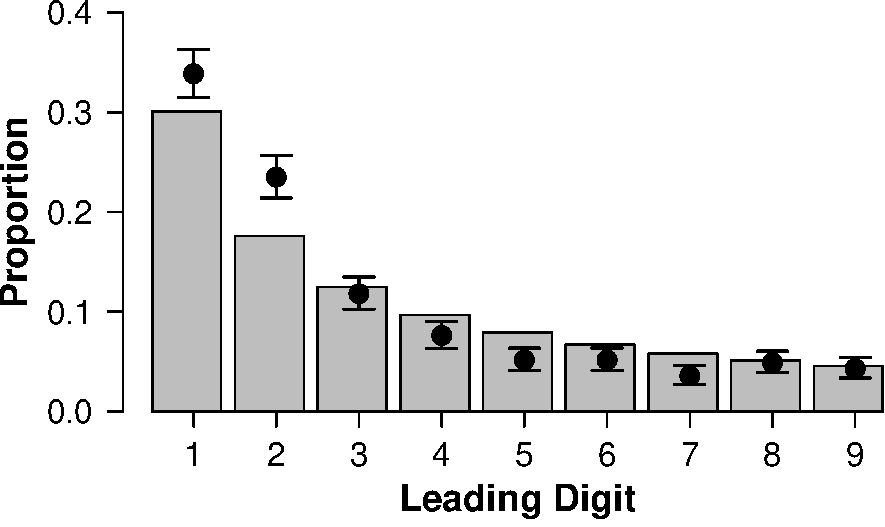
\includegraphics{Rpackage_paper_files/figure-latex/benford-1.pdf}
\caption{\label{fig:benford}The bargraph displays the expected proportions of leading digits according to Benford's law. The black dots indicate for the actual fiscal statistics from Greece the posterior estimates for the proportion of leading digits and the corresponding 95\% credible intervals. Only three out of nine estimates cover the expected proportions.}
\end{figure}

\hypertarget{discussion}{%
\subsubsection{Discussion}\label{discussion}}

In this example we tested the data quality of Greek fiscal data in the years 1999 to 2009 by conducting three variations of a Bayesian Benford test. More precise, we evaluated the null hypothesis that the data conform to Benfords law. We tested this hypothesis against three alternatives. The first alternative hypothesis, \(\mathcal{H}_e\) relaxed the constraints imposed by the null hypothesis and let all model parameters free to vary. The second alternative hypothesis, \(\mathcal{H}_{r1}\) predicted a decreasing trend in the proportion of leading digits. The third alternative hypothesis \(\mathcal{H}_{r2}\) predicted a trend that Hill (1988) observed in manipulated data. Our result suggest that the leading digits in the fiscal statistics do not follow a Benford distribution; in fact, we collected extreme evidence against Benford's law compared to all two out of three of the alternative hypotheses. When comparing the alternative hypotheses directly to each other, the data show most evidence in favor for a decreasing trend. A Benford test when used in to check fiscal statements can be a helpful tool to detect poor data quality and suspicious numbers. In follow-up checks of these numbers, it could then be examined for instance, whether financial statements were actually materially misstated (by, for instance, rounding up or down numbers, avoiding certain thresholds etc., Nigrini, 2019).

\hypertarget{example-2-prevalence-of-statistical-reporting-errors}{%
\subsection{Example 2: Prevalence of Statistical Reporting Errors}\label{example-2-prevalence-of-statistical-reporting-errors}}

In any scientific article that uses null hypothesis significance testing, there is a chance that the reported test statistic and degrees of freedom, do not match the reported \(p\)-value. In most cases this is because researchers copy the relevant test statistics by hand into their articles and there are no automatic checks to detect these mistakes. Therefore, Epskamp and Nuijten (2014) developed the R package \texttt{statcheck}, which only requires the PDF of a given scientific article to detect these reporting errors automatically and efficiently. This package allowed Nuijten et al. (2016) to get an overview about the prevalence of statistical reporting errors in the field of psychology. In total, the authors investigated a sample of \(30,717\) articles (which translates to over a quarter of a million \(p\)-values) published in eight major psychological journals between 1985 to 2013: \emph{Developmental Psychology} (DP), the \emph{Frontiers in Psychology} (FP), the \emph{Journal of Applied Psychology} (JAP), the \emph{Journal of Consulting and Clinical Psychology} (JCCP), \emph{Journal of Experimental Psychology: General} (JEPG), the \emph{Journal of Personality and Social Psychology} (JPSP), the \emph{Public Library of Science} (PLoS), \emph{Psychological Science} (PS).

Besides the overall prevalence of statistical reporting errors across these journals, the authors were interested whether there is a higher prevalence for reporting inconsistencies in certain subfields in psychology compared to others. In this context the assumption was raised that there exists a relationship between the prevalence for reporting inconsistencies and questionable research practices. Specifically, the authors argued that besides honest mistakes when transferring the test statistics into the manuscript, statistical reporting error occur when authors misreport \(p\)-values, for instance, by incorrectly rounding them down below \(0.05\). Based on this assumption Nuijten et al. (2016) predicted that the proportion of statistical reporting errors should be highest in articles published in the \emph{Journal of Personality and Social Psychology} (JPSP), compared to other journals, since researchers in social psychology were shown to have the highest prevalence for questionable research practices (John, Loewenstein, \& Prelec, 2012). Specifically, John et al. (2012) found that researchers from the area of social psychology assessed questionable research practices both as more defensible and more applicable for their research compared to other research areas in psychology.

\hypertarget{data-and-hypothesis-1}{%
\subsubsection{Data and Hypothesis}\label{data-and-hypothesis-1}}

We will use the original data published in the article by Nuijten et al. (2016) and which we included under the name of \texttt{journals} in the package \textbf{multibridge}.

\begin{Shaded}
\begin{Highlighting}[]
\CommentTok{# load the package and data}
\KeywordTok{data}\NormalTok{(journals)}
\end{Highlighting}
\end{Shaded}

The hypothesis of interest,\(\mathcal{H}_r\), formulated by Nuijten et al. (2016) states that the prevalence for statistical reporting errors for articles published in social psychology journals (i.e., JPSP) is higher than for articles published in other journals. We will test this hypothesis against the the null hypothesis \(\mathcal{H}_0\) that all journals have the same prevalence for statistical reporting errors. In this example, the parameter vector of the binomial success probabilities, \(\boldsymbol{\theta}\), it reflects the probabilities of a statistical reporting error in one of the 8 journals. Thus, we can formalize the discussed hypotheses as follows:

\begin{align*}
    \mathcal{H}_r &: \theta_{\text{DP}}, \theta_{\text{FP}}, \theta_{\text{JAP}} , \theta_{\text{JCCP}} , \theta_{\text{JEPG}} , \theta_{\text{PLoS}}, \theta_{\text{PS}}) < \theta_{\text{JPSP}} \\
    \mathcal{H}_0 &: \theta_{\text{DP}} =  \theta_{\text{FP}} =  \cdots = \theta_{\text{JPSP}}.
\end{align*}

\hypertarget{method-1}{%
\subsubsection{Method}\label{method-1}}

As before, we can compute \(\text{BF}_{0r}\) through the transitivity of the Bayes factor, that is, \(\text{BF}_{r0} = \text{BF}_{re} \times \text{BF}_{e0}\). The Bayes factor \(\text{BF}_{e0}\) can be computed by using the \texttt{binomBfEquality()} function.

\begin{Shaded}
\begin{Highlighting}[]
\CommentTok{# Since percentages are rounded to two decimal values, we round the articles}
\CommentTok{# with an error to receive integer values}
\NormalTok{x <-}\StringTok{ }\KeywordTok{round}\NormalTok{(journals}\OperatorTok{$}\NormalTok{articles_with_NHST  }\OperatorTok{*}\StringTok{ }
\StringTok{             }\NormalTok{(journals}\OperatorTok{$}\NormalTok{perc_articles_with_errors}\OperatorTok{/}\DecValTok{100}\NormalTok{))}
\CommentTok{# Total number of articles}
\NormalTok{n <-}\StringTok{ }\NormalTok{journals}\OperatorTok{$}\NormalTok{articles_with_NHST}

\CommentTok{# Prior specification}
\CommentTok{# We assign a uniform beta distribution to each binomial propotion}
\NormalTok{a <-}\StringTok{ }\KeywordTok{rep}\NormalTok{(}\DecValTok{1}\NormalTok{, }\DecValTok{8}\NormalTok{)}
\NormalTok{b <-}\StringTok{ }\KeywordTok{rep}\NormalTok{(}\DecValTok{1}\NormalTok{, }\DecValTok{8}\NormalTok{)}

\NormalTok{results_He_H0   <-}\StringTok{ }\KeywordTok{binomBfEquality}\NormalTok{(}\DataTypeTok{x=}\NormalTok{x, }\DataTypeTok{n=}\NormalTok{n, }\DataTypeTok{a=}\NormalTok{a, }\DataTypeTok{b=}\NormalTok{b)}
\NormalTok{eq_bayesfactors <-}\StringTok{ }\NormalTok{results_He_H0}\OperatorTok{$}\NormalTok{bf}
\end{Highlighting}
\end{Shaded}

The data suggest that the null hypothesis is highly unlikely; we collected extreme evidence against the null hypothesis with a log Bayes factor \(\text{log}(\text{BF}_{0e})\) of -156.

To compute the Bayes factor \(\text{BF}_{re}\) we need to specify (1) a vector with observed successes, and (2) a vector containing the total number of observations, (3) the informed hypothesis, (4) a vector with prior parameters alpha for each binomial proportion, (5) a vector with prior parameters beta for each binomial proportion, and (6) the categories of interest (i.e., journal names). With this information, we can now conduct the analysis with the function \texttt{binomBfInformed}.

\begin{Shaded}
\begin{Highlighting}[]
\CommentTok{# Specifying the informed Hypothesis}
\NormalTok{Hr <-}\StringTok{ }\KeywordTok{c}\NormalTok{(}\StringTok{'JAP , PS , JCCP , PLOS , DP , FP , JEPG < JPSP'}\NormalTok{)}

\CommentTok{# Categories of interest}
\NormalTok{journal_names <-}\StringTok{ }\NormalTok{journals}\OperatorTok{$}\NormalTok{journal}

\CommentTok{# Execute the analysis}
\NormalTok{results_Hr_He <-}\StringTok{ }\KeywordTok{binomBfInformed}\NormalTok{(}\DataTypeTok{x =}\NormalTok{ x, }\DataTypeTok{n =}\NormalTok{ n, }\DataTypeTok{Hr =}\NormalTok{ Hr, }\DataTypeTok{a =}\NormalTok{ a, }\DataTypeTok{b =}\NormalTok{ b,}
                               \DataTypeTok{factor_levels =}\NormalTok{ journal_names,}
                               \DataTypeTok{bf_type =} \StringTok{'BFre'}\NormalTok{, }\DataTypeTok{seed =} \DecValTok{2020}\NormalTok{)}
\end{Highlighting}
\end{Shaded}

We collected moderate evidence for the informed
hypothesis. Specifically, the results suggest that the data
are 7.43 more likely under
the informed hypothesis than under the hypothesis that all parameters are
free to vary. As final step, we compare the informed and the null hypothesis directly
with each other.

\begin{Shaded}
\begin{Highlighting}[]
\NormalTok{BFre <-}\StringTok{ }\NormalTok{results_Hr_He}\OperatorTok{$}\NormalTok{bf_list}\OperatorTok{$}\NormalTok{bf}\OperatorTok{$}\NormalTok{BFre}
\NormalTok{BFe0 <-}\StringTok{ }\NormalTok{eq_bayesfactors[[}\StringTok{'BFe0'}\NormalTok{]]}
\NormalTok{BFr0 <-}\StringTok{ }\NormalTok{BFre }\OperatorTok{*}\StringTok{ }\NormalTok{BFe0}
\end{Highlighting}
\end{Shaded}

The Bayes factor \(log(\text{BF}_{r0})\) suggests extreme evidence for the informed hypothesis; \(\text{log}(\text{BF}_{r0}) =\) 158.

\hypertarget{discussion-1}{%
\subsubsection{Discussion}\label{discussion-1}}

In this example we tested whether the prevalence for statistical reporting errors for articles published in social psychology journals (i.e., JPSP) is higher than for articles published in other journals. We tested this hypothesis against the null hypothesis that the prevalence for statistical reporting errors is equal across all journals. The resulting Bayes factor of \(\text{log}(\text{BF}_{r0}) =\) 5.48e+68 provides extreme evidence for the informed hypothesis. However, this result should be interpreted with caution and be considered more differentiated. It seems that the result is above all an indication that the null hypothesis is highly misspecified and that the prevalence for a statistical reporting error varies greatly from journal to journal. Evidence that JPSP stands out and has a higher prevalence than the other journals is relatively small; the data provided only moderate evidence against the encompassing hypotheses.

\hypertarget{summary}{%
\section{Summary}\label{summary}}

The \texttt{R} package \textbf{multibridge} facilitates the computation of Bayes factors for informed hypotheses in multinomial models. The underlying algorithm is based on a bridge sampling routine that was recently developed and was shown to be more efficient and produces more reliable estimates than comparable methods. The current version of \textbf{multibridge}, the user can specify hypotheses that feature equality constraints, inequality constraints, and free parameters as well as mixtures between them. The core functions of the software package were illustrated with two empirical examples. The \textbf{multibridge} package is under continuous development. In future versions of the package, we aim to implement methods that allow for the evaluation of hierarchical multinomial models. In addition, we want to allow users to specify order constraints that are more complex, including hypotheses on the size ratios of the parameters of interest or the difference between category proportions.

\hypertarget{references}{%
\section{References}\label{references}}

\begingroup
\setlength{\parindent}{-0.5in}
\setlength{\leftskip}{0.5in}

\hypertarget{refs}{}
\leavevmode\hypertarget{ref-benford1938law}{}%
Benford, F. (1938). The law of anomalous numbers. \emph{Proceedings of the American Philosophical Society}, 551--572.

\leavevmode\hypertarget{ref-bennett1976efficient}{}%
Bennett, C. H. (1976). Efficient estimation of free energy differences from Monte Carlo data. \emph{Journal of Computational Physics}, \emph{22}, 245--268.

\leavevmode\hypertarget{ref-damien2001sampling}{}%
Damien, P., \& Walker, S. G. (2001). Sampling truncated normal, beta, and gamma densities. \emph{Journal of Computational and Graphical Statistics}, \emph{10}, 206--215.

\leavevmode\hypertarget{ref-durtschi2004effective}{}%
Durtschi, C., Hillison, W., \& Pacini, C. (2004). The effective use of benford's law to assist in detecting fraud in accounting data. \emph{Journal of Forensic Accounting}, \emph{5}, 17--34.

\leavevmode\hypertarget{ref-epskamp2014statcheck}{}%
Epskamp, S., \& Nuijten, M. (2014). Statcheck: Extract statistics from articles and recompute p values (R package version 1.0.0.).

\leavevmode\hypertarget{ref-europeanCommision2004}{}%
European Commision. (2004). Report by Eurostat on the revision of the Greek government deficit and debt figures. Eurostat Report, \url{https://ec.europa.eu/eurostat/web/products-eurostat-news/-/GREECE}.

\leavevmode\hypertarget{ref-europeanCommision2010}{}%
European Commision. (2010). Report on Greek government deficit and debt statistics. Eurostat Report, \url{https://ec.europa.eu/eurostat/web/products-eurostat-news/-/COM_2010_REPORT_GREEK}.

\leavevmode\hypertarget{ref-frigyik2010introduction}{}%
Frigyik, B. A., Kapila, A., \& Gupta, M. R. (2010). \emph{Introduction to the Dirichlet distribution and related processes}. Department of Electrical Engineering, University of Washington.

\leavevmode\hypertarget{ref-gronau2017tutorial}{}%
Gronau, Q. F., Sarafoglou, A., Matzke, D., Ly, A., Boehm, U., Marsman, M., \ldots{} Steingroever, H. (2017). A tutorial on bridge sampling. \emph{Journal of Mathematical Psychology}, \emph{81}, 80--97.

\leavevmode\hypertarget{ref-gronau2017bridgesampling}{}%
Gronau, Q. F., Singmann, H., \& Wagenmakers, E. (2020). Bridgesampling: An R package for estimating normalizing constants. \emph{Journal of Statistical Software, Articles}, \emph{92}(10), 1--29.

\leavevmode\hypertarget{ref-gu2019bain}{}%
Gu, X., Hoijtink, H., Mulder, J., \& Rosseel, Y. (2019). Bain: A program for bayesian testing of order constrained hypotheses in structural equation models. \emph{Journal of Statistical Computation and Simulation}, \emph{89}, 1526--1553.

\leavevmode\hypertarget{ref-gu2014bayesian}{}%
Gu, X., Mulder, J., Deković, M., \& Hoijtink, H. (2014). Bayesian evaluation of inequality constrained hypotheses. \emph{Psychological Methods}, \emph{19}, 511--527.

\leavevmode\hypertarget{ref-heck2019multinomial}{}%
Heck, D. W., \& Davis-Stober, C. P. (2019). Multinomial models with linear inequality constraints: Overview and improvements of computational methods for Bayesian inference. \emph{Journal of Mathematical Psychology}, \emph{91}, 70--87.

\leavevmode\hypertarget{ref-hill1988random}{}%
Hill, T. P. (1988). Random-number guessing and the first digit phenomenon. \emph{Psychological Reports}, \emph{62}, 967--971.

\leavevmode\hypertarget{ref-hill1995statistical}{}%
Hill, T. P. (1995). A statistical derivation of the significant-digit law. \emph{Statistical Science}, 354--363.

\leavevmode\hypertarget{ref-hoijtink2011informative}{}%
Hoijtink, H. (2011). \emph{Informative hypotheses: Theory and practice for behavioral and social scientists}. Boca Raton, FL: Chapman \& Hall/CRC.

\leavevmode\hypertarget{ref-hoijtink2008bayesian}{}%
Hoijtink, H., Klugkist, I., \& Boelen, P. (Eds.). (2008). \emph{Bayesian evaluation of informative hypotheses}. New York: Springer Verlag.

\leavevmode\hypertarget{ref-jeffreys1935some}{}%
Jeffreys, H. (1935). Some tests of significance, treated by the theory of probability. In \emph{Proceedings of the Cambridge Philosophy Society} (Vol. 31, pp. 203--222).

\leavevmode\hypertarget{ref-john2012measuring}{}%
John, L. K., Loewenstein, G., \& Prelec, D. (2012). Measuring the prevalence of questionable research practices with incentives for truth telling. \emph{Psychological Science}, \emph{23}, 524--532.

\leavevmode\hypertarget{ref-kass1995bayes}{}%
Kass, R. E., \& Raftery, A. E. (1995). Bayes factors. \emph{Journal of the American Statistical Association}, \emph{90}, 773--795.

\leavevmode\hypertarget{ref-klugkist2005bayesian}{}%
Klugkist, I., Kato, B., \& Hoijtink, H. (2005). Bayesian model selection using encompassing priors. \emph{Statistica Neerlandica}, \emph{59}, 57--69.

\leavevmode\hypertarget{ref-meng1996simulating}{}%
Meng, X.-L., \& Wong, W. H. (1996). Simulating ratios of normalizing constants via a simple identity: A theoretical exploration. \emph{Statistica Sinica}, \emph{6}, 831--860.

\leavevmode\hypertarget{ref-mulder2014prior}{}%
Mulder, J. (2014). Prior adjusted default Bayes factors for testing (in) equality constrained hypotheses. \emph{Computational Statistics \& Data Analysis}, \emph{71}, 448--463.

\leavevmode\hypertarget{ref-mulder2016bayes}{}%
Mulder, J. (2016). Bayes factors for testing order--constrained hypotheses on correlations. \emph{Journal of Mathematical Psychology}, \emph{72}, 104--115.

\leavevmode\hypertarget{ref-mulder2012biems}{}%
Mulder, J., Hoijtink, H., Leeuw, C. de, \& others. (2012). BIEMS: A Fortran 90 program for calculating Bayes factors for inequality and equality constrained models. \emph{Journal of Statistical Software}, \emph{46}, 1--39.

\leavevmode\hypertarget{ref-mulder2009bayesian}{}%
Mulder, J., Klugkist, I., van de Schoot, R., Meeus, W. H. J., Selfhout, M., \& Hoijtink, H. (2009). Bayesian model selection of informative hypotheses for repeated measurements. \emph{Journal of Mathematical Psychology}, \emph{53}, 530--546.

\leavevmode\hypertarget{ref-newcomb1881note}{}%
Newcomb, S. (1881). Note on the frequency of use of the different digits in natural numbers. \emph{American Journal of Mathematics}, \emph{4}, 39--40.

\leavevmode\hypertarget{ref-nigrini2012benford}{}%
Nigrini, M. (2012). \emph{Benford's Law: Applications for forensic accounting, auditing, and fraud detection} (Vol. 586). Hoboken, New Jersey: John Wiley \& Sons.

\leavevmode\hypertarget{ref-nigrini2019patterns}{}%
Nigrini, M. J. (2019). The patterns of the numbers used in occupational fraud schemes. \emph{Managerial Auditing Journal}, \emph{34}, 602--622.

\leavevmode\hypertarget{ref-nigrini1997use}{}%
Nigrini, M. J., \& Mittermaier, L. J. (1997). The use of benford's law as an aid in analytical procedures. \emph{Auditing}, \emph{16}, 52.

\leavevmode\hypertarget{ref-nuijten2016prevalence}{}%
Nuijten, M. B., Hartgerink, C. H., Assen, M. A. van, Epskamp, S., \& Wicherts, J. M. (2016). The prevalence of statistical reporting errors in psychology (1985--2013). \emph{Behavior Research Methods}, \emph{48}, 1205--1226.

\leavevmode\hypertarget{ref-overstall2010default}{}%
Overstall, A. M., \& Forster, J. J. (2010). Default Bayesian model determination methods for generalised linear mixed models. \emph{Computational Statistics \& Data Analysis}, \emph{54}, 3269--3288.

\leavevmode\hypertarget{ref-rauch2011fact}{}%
Rauch, B., Göttsche, M., Brähler, G., \& Engel, S. (2011). Fact and fiction in EU-governmental economic data. \emph{German Economic Review}, \emph{12}, 243--255.

\leavevmode\hypertarget{ref-sarafoglou2020evaluatingPreprint}{}%
Sarafoglou, A., Haaf, J. M., Ly, A., Gronau, Q. F., Wagenmakers, E., \& Marsman, M. (2020). Evaluating multinomial order restrictions with bridge sampling. \emph{PsyArXiv}. Retrieved from \url{https://psyarxiv.com/bux7p/}

\leavevmode\hypertarget{ref-stan2020}{}%
Stan Development Team. (2020). \emph{Stan modeling language user's guide and reference manual, version 2.23.0}. R Foundation for Statistical Computing. Retrieved from \url{http://mc-stan.org/}

\endgroup

\hypertarget{appendix-transforming-an-ordered-probability-vector-to-the-real-line}{%
\subsection{Appendix: Transforming An Ordered Probability Vector To The Real Line}\label{appendix-transforming-an-ordered-probability-vector-to-the-real-line}}

Since we choose the multivariate normal as proposal distribution, the mapping between the proposal and target distribution requires us to move \(\boldsymbol{\theta}\) to the real line. Crucially this transformation needs to retain the inequality constraints imposed on the parameters. To achieve this goal, \textbf{multibridge} uses a probit transformation which subsequently transforms the elements in \(\boldsymbol{\theta}\) moving from its lowest to its highest value. In the binomial model, we move all elements in \(\boldsymbol{\theta}\) to the real line and thus construct a new vector \(\boldsymbol{y} \in \mathbb{R}^{K}\). For multinomial models, however, it follows from the unit constraint that the vector \(\boldsymbol{\theta}\) is completely determined by its first \(K - 1\) elements of \(\boldsymbol{\theta}: \theta_1 \leq \theta_2 \leq \cdots \leq 1 - \sum_{k = 1}^K \theta_k\). Hence, for the transformation we will only consider the first \(K - 1\) elements of \(\boldsymbol{\theta}\) and we will transform them to \(K - 1\) elements of a new vector \(\boldsymbol{y} \in \mathbb{R}^{K - 1}\).

Let \(\phi\) denote the density of a normal variable with a mean of zero and a variance of one, \(\Phi\) denote its cumulative density function, and \(\Phi^{-1}\) denote the inverse cumulative density function. Then for each element \(\theta_k\), the transformation is
\[\xi_k = \Phi^{-1}\left(\frac{\theta_k - l_k}{u_k - l_k}\right),\]
The inverse transformation is given by
\[\theta_k = (u_k - l_k) \Phi(\xi_k) + l_k.\]
The Jacobian of this transformation is:
\[\left|J\right| = \prod_{k = 1}^{K - 1}  \left(u_k - l_k \right) \phi(\xi_k).\]

To perform the transformations, we thus need to determine the lower bound \(l_k\) and the upper bound \(u_k\) of each \(\theta_k\). Assuming \(\theta_{k-1} < \theta_{k}\) for \(k \in \{1 \cdots, K\}\) the lower bound for any element in \(\boldsymbol{\theta}\) is defined as

\begin{align*}
  l_k = \left.
  \begin{cases}
      0 & \text{if } k = 1 \\
      \theta_{k - 1} & \text{if } 1 < k < K.
  \end{cases}
    \right.
\end{align*}

This definition holds for both binomial models and multinomial models. Differences in these two models appear only when determining the upper bound for each parameter, since parameters in a multinomial models are unit constrained. For binomial models, the upper bound for each \(\theta_k\) is simply \(1\). For multinomial models, however, the upper bound for each \(\theta_k\) depends on the size of smaller elements as well as on the number of remaining larger elements in \(\boldsymbol{\theta}\). To determine the upper bound for multinomial parameters we are using a stick-breaking method (Frigyik, Kapila, \& Gupta, 2010; Stan Development Team, 2020). The stick-breaking approach represents \(\boldsymbol{\theta}\) as unit-length stick which we subsequently divide into \(K\) elements. By this definition, the upper bound or any \(\theta_k\) is:

\begin{align}
\label{Eq:upperBound}
  u_k = \left.
  \begin{cases}
      \cfrac{1}{K} & \text{if } k = 1 \\
      \cfrac{1 - \sum_{i < k} \theta_i}{ERS} & \text{if } 1 < k < K,
  \end{cases}
    \right.
\end{align}
where \(1 - \sum_{i < k} \theta_i\) represents the length of the remaining stick, that is, the proportion of the unit-length stick that still needs to be divided among the remaining elements in \(\boldsymbol{\theta}\). The elements in the remaining stick are denoted as \(ERS\), and are computed as follows: \[ERS = K - 1 + k\].

The transformations outlined above are suitable for binomial and multinomial models featuring hypotheses in which all parameters are inequality constrained. However, when hypotheses feature a combination of equality and inequality constrained parameters, as well as parameters that are free to vary we need to modify the formula to compute the upper and lower bounds:

\begin{align}
  l_k = \left.
  \begin{cases}
      0 & \text{if } k = 1 \\
      \frac{\theta_{k - 1}}{e_{k-1}} \times e_k & \text{if } 1 < k < K,
  \end{cases}
    \right.
\end{align}
where \(e_{k-1}\) refers to the number of equality constrained parameters that are collapsed in \(\theta_{k - 1}\).

The upper bound for parameters in the binomial models still remains \(1\). For multinomial models, the upper bound is then defined as:

\begin{align}
  u_k = \left.
  \begin{cases}
      \cfrac{1}{K} - (f_k \times l_k) & \text{if } k = 1 \\
     \left( \cfrac{1 - \sum_{i < k} \theta_i}{ERS} - (f_k \times l_k) \right) \times e_k & \text{if } 1 < k < K \text{ and } u_k \geq \text{max}(\theta_{i < k}), \\
    \left( 2 \times \left( \cfrac{1 - \sum_{i < k} \theta_i}{ERS} - (f_k \times l_k) \right) - \text{max}(\theta_{i < k}) \right)  \times e_k & \text{if } 1 < k < K \text{ and } u_k < \text{max}(\theta_{i < k}),
  \end{cases}
    \right.
\end{align}
where \(f_k\) represents the number of free parameters that share common upper and lower bounds. The elements in the remaining stick are then computed as follows \[ERS = e_k + \sum_{j > k} e_j \times f_j\].The rationale behind these modifications will be described in more detail in the following sections. In \textbf{multibridge} information that is relevant for the transformation of the parameter vectors is stored in the generated \texttt{restriction\_list} which is returned by the main functions \texttt{binomBfInformed} and \texttt{multBfInformed} but can also be generated separately with the function \texttt{generateRestrictionList}. This restriction list features the sublist \texttt{inequality\_constraints} which encodes the number of equality constraints collapsed in each parameter in \texttt{nr\_mult\_equal}. Similarly the number of free parameters that share a common bounds are encoded under \texttt{nr\_mult\_free}.

\hypertarget{equality-constrained-parameters}{%
\paragraph{Equality Constrained Parameters}\label{equality-constrained-parameters}}

When informed hypotheses feature a mix of equality and inequality constrained parameters, we collapse in the constrained prior and posterior distributions all equality constrained parameters into one category. When transforming the samples from these distributions, we need to account for the fact that inequality constraints on the collapsed parameters might not hold even though the constraint is valid under the original parameter values. For instance, for \(\theta_1 = \theta_2 = \theta_3 \leq \theta_4 \leq \theta_5\), where the elements in \(\boldsymbol{\theta}\) take the values \((0.15, 0.15, 0.15, 0.25, 0.3)\), the inequality constraint does not hold for the collapsed parameters (i.e., \(\theta^* \nless \theta_4 \leq \theta_5\) since \(0.45 \nleq 0.25 \leq 0.3\)). For these cases, the upper and lower bounds for the parameters need to be adjusted as follows:
\begin{align}
  l_k = \left.
  \begin{cases}
      0 & \text{if } k = 1 \\
      \frac{\theta_{k - 1}}{e_{k-1}} \times e_k & \text{if } 1 < k < K,
  \end{cases}
    \right.
\end{align}
where \(e_{k-1}\) and \(e_k\) refer to the number of equality constrained parameters that are collapsed in \(\theta_{k - 1}\) and \(\theta_{k}\), respectively. The upper bound is defined as

\begin{align}
  u_k = \left.
  \begin{cases}
      \cfrac{1}{ERS} \times e_k & \text{if } k = 1 \\
      \cfrac{1 - \sum_{i < k} \theta_i}{ERS} \times e_k & \text{if } 1 < k < K,
  \end{cases}
    \right.
\end{align}
where \(1 - \sum_{i < k} \theta_i\) represents the length of the remaining stick and the number of elements in the remaining stick are computed as follows: \(ERS = \sum_k^{K} e_k\). The upper bound is then multiplied by the number of equality constrained parameters within the current constraint.

Concretely, for the constraint above, that is \(\theta^* \leq \theta_4\), the lower bound for \(\theta^*\) would be \(0\). The upper bound is computed by taking account the number of equality constrained parameters, such that \(u_k = \nicefrac{1}{5} \times 3 = 0.6\). For \(\theta_4\) the lower bound is \(\nicefrac{\theta^*}{3} = 0.15\), since \(3\) parameters are collapsed in \(\theta^*\). The upper bound for \(\theta_4\) is then \(\cfrac{(1 - \theta^*)}{2} = 0.275\) and \(\theta_5\) is \(1 - \theta^* - \theta_4 = 1 - 0.45 - 0.25 = 0.3\).

\hypertarget{corrections-for-free-parameters}{%
\paragraph{Corrections for Free Parameters}\label{corrections-for-free-parameters}}

Different adjustments are required for a sequence of inequality constraint parameters that have shared upper and lower bounds, but can vary freely within certain upper and lower bounds. For instance, the hypothesis \[\mathcal{H}_r: \theta_1 < \theta_2, \theta_3\] specifies that \(\theta_2\) and \(\theta_3\) have the shared lower bound \(\theta_1\) and the shared upper bound \(1\), however, \(\theta_2\) can be larger than \(\theta_3\) or vice versa. To integrate these cases within the stick-breaking approach one must account for these potential changes of order. For these cases, the lower bounds for the parameters remain unchanged, however the upper bounds need to be adjusted as follows:
\begin{align}
  u_k = \left.
  \begin{cases}
      \cfrac{1}{K} - (f_k \times l_k) & \text{if } k = 1 \\
      \cfrac{1 - \sum_{i < k} \theta_i}{ERS} - (f_k \times l_k) & \text{if } 1 < k < K,
  \end{cases}
    \right.
\end{align}

where \(f_k\) represents the number of free parameters that share common upper and lower bounds. Here, the number of elements in the remaining stick are computed as follows: \(ERS = 1 + \sum_{j > k} f_j\). Subtracting the lower bound for the remaining free parameters from the upper bound of the current parameter secures a minimum stick-length for the remaining free parameters to comply with the constraint. A further correction is required, if a preceding free parameter (i.e., a free parameter that was already accounted for in the stick) is larger than the upper bound of the current parameter. In that case, we need we subtract the difference between the largest preceding free parameter in the sequence with the current upper bound. Thus if \(u_k < \text{max}(\theta_{i < k})\), the upper bound becomes:
\begin{align}
u_k &= u_k - (\text{max}(\theta_{i < k}) - u_k)\\
    &= 2 \times u_k - \text{max}(\theta_{i < k}).
\end{align}

To outline when such a correction is necessary, consider the constraint \(\theta_1 \leq \theta_2, \theta_3 \leq \theta_4,\) where the elements in \(\boldsymbol{\theta}\) take on the values \((0.1, 0.35, 0.15, 0.40)\). When transforming the parameters, the lower bound for \(\theta_1\) is \(0\), the upper bound \(\nicefrac{1}{4}\). The parameters \(\theta_2\) and \(\theta_3\) share the same lower bound, which is, \(\theta_1 = 0.1\). The upper bound for \(\theta_2\), is the length of the remaining stick divided by the elements of the remaining stick, that is, \(\nicefrac{0.9}{2} = 0.45\). From the resulting upper bound, we subtract the lower bound for the remaining free parameters of the sequence, which yields an upper bound for \(\theta_2\) of \(0.45 - 0.1 = 0.35\). Since \(\theta_2\) is the first free parameter in the sequence that is evaluated an additional downward correction is not necessary. The upper bound for \(\theta_3\) is \((1 - 0.1 - 0.35)/2 = 0.275\). However, if \(\theta_3\) would actually take on the value \(0.275\), \(\theta_4\) would need to be \(0.275\) too, which would violate the constraint (i.e., \(0.1 \leq 0.35, 0.275 \nleq 0.275\)). Therefore, we apply the additional correction, such that
\begin{align}
  u_k &= 2 \times u_k - \text{max}(\theta_{i < k}) \\
      &= 2 \times 0.275 - 0.35 \\
      &= 0.2,
\end{align}
which secures the proper ordering for the remainder of the parameters, since \(\theta_4 = 0.2\) would yield \(0.1 \leq 0.35, 0.2 \leq 0.35\).


\end{document}
